\begin{figure}[h!]
	\begin{minipage}{0.4\linewidth}
	\centering
	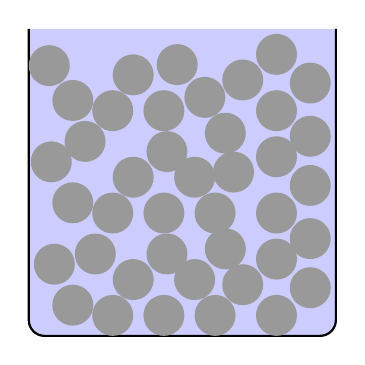
\begin{tikzpicture}[scale = 1.3]
		\filldraw[fill =blue!20,thick,  rounded corners = 2mm] (0, 0) -- (0, -3) -- (3, -3) -- (3, 0); 
		\fill[black!40] (0.25, -2.3) circle (2mm);
		\fill[black!40] (0.65, -2.2) circle (2mm);
		\fill[black!40] (1.35, -2.2) circle (2mm);
		\fill[black!40] (0.43, -2.7) circle (2mm);
		\fill[black!40] (0.82, -2.8) circle (2mm);
		\fill[black!40] (1.32, -2.8) circle (2mm);
		\fill[black!40] (1.92, -2.15) circle (2mm);
		\fill[black!40] (1.82, -2.8) circle (2mm);
		\fill[black!40] (2.42, -2.8) circle (2mm);
		\fill[black!40] (1.02, -2.45) circle (2mm);
		\fill[black!40] (1.62, -2.45) circle (2mm);
		\fill[black!40] (2.09, -2.5) circle (2mm);
		\fill[black!40] (2.75, -2.53) circle (2mm);
		\fill[black!40] (2.42, -2.25) circle (2mm);
		\fill[black!40] (2.75, -2.05) circle (2mm);
		%%%%%%%%%
		\fill[black!40] (0.22, -1.3) circle (2mm);
		\fill[black!40] (0.55, -1.1) circle (2mm);
		\fill[black!40] (0.43, -1.7) circle (2mm);
		\fill[black!40] (0.82, -1.8) circle (2mm);
		\fill[black!40] (1.32, -1.8) circle (2mm);
		\fill[black!40] (1.35, -1.2) circle (2mm);
		\fill[black!40] (1.82, -1.8) circle (2mm);
		\fill[black!40] (2.42, -1.8) circle (2mm);
		\fill[black!40] (1.02, -1.45) circle (2mm);
		\fill[black!40] (1.62, -1.45) circle (2mm);
		\fill[black!40] (2, -1.4) circle (2mm);
		\fill[black!40] (2.75, -1.53) circle (2mm);
		\fill[black!40] (2.42, -1.25) circle (2mm);
		\fill[black!40] (2.75, -1.05) circle (2mm);
		%%%%%%%%%
		\fill[black!40] (0.2, -0.36) circle (2mm);
		\fill[black!40] (0.43, -0.7) circle (2mm);
		\fill[black!40] (0.82, -0.8) circle (2mm);
		\fill[black!40] (1.32, -0.8) circle (2mm);
		\fill[black!40] (1.72, -0.67) circle (2mm);
		\fill[black!40] (1.92, -1.02) circle (2mm);
		\fill[black!40] (2.42, -0.8) circle (2mm);
		\fill[black!40] (1.02, -0.45) circle (2mm);
		\fill[black!40] (1.45, -0.35) circle (2mm);
		\fill[black!40] (2.09, -0.5) circle (2mm);
		\fill[black!40] (2.75, -0.53) circle (2mm);
		\fill[black!40] (2.42, -0.25) circle (2mm);
	\end{tikzpicture}
	\end{minipage}
	\begin{minipage}{0.2\linewidth}
		\begin{center}
			$\rightarrow$
		\end{center}
	\end{minipage}
	\begin{minipage}{0.4\linewidth}
	\centering
	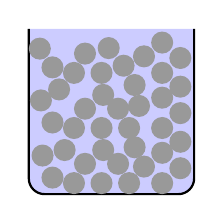
\begin{tikzpicture}[scale = 0.7]
		\filldraw[fill =blue!20,thick,  rounded corners = 2mm] (0, 0) -- (0, -3) -- (3, -3) -- (3, 0); 
		\fill[black!40] (0.25, -2.3) circle (2mm);
		\fill[black!40] (0.65, -2.2) circle (2mm);
		\fill[black!40] (1.35, -2.2) circle (2mm);
		\fill[black!40] (0.43, -2.7) circle (2mm);
		\fill[black!40] (0.82, -2.8) circle (2mm);
		\fill[black!40] (1.32, -2.8) circle (2mm);
		\fill[black!40] (1.92, -2.15) circle (2mm);
		\fill[black!40] (1.82, -2.8) circle (2mm);
		\fill[black!40] (2.42, -2.8) circle (2mm);
		\fill[black!40] (1.02, -2.45) circle (2mm);
		\fill[black!40] (1.62, -2.45) circle (2mm);
		\fill[black!40] (2.09, -2.5) circle (2mm);
		\fill[black!40] (2.75, -2.53) circle (2mm);
		\fill[black!40] (2.42, -2.25) circle (2mm);
		\fill[black!40] (2.75, -2.05) circle (2mm);
		%%%%%%%%%
		\fill[black!40] (0.22, -1.3) circle (2mm);
		\fill[black!40] (0.55, -1.1) circle (2mm);
		\fill[black!40] (0.43, -1.7) circle (2mm);
		\fill[black!40] (0.82, -1.8) circle (2mm);
		\fill[black!40] (1.32, -1.8) circle (2mm);
		\fill[black!40] (1.35, -1.2) circle (2mm);
		\fill[black!40] (1.82, -1.8) circle (2mm);
		\fill[black!40] (2.42, -1.8) circle (2mm);
		\fill[black!40] (1.02, -1.45) circle (2mm);
		\fill[black!40] (1.62, -1.45) circle (2mm);
		\fill[black!40] (2, -1.4) circle (2mm);
		\fill[black!40] (2.75, -1.53) circle (2mm);
		\fill[black!40] (2.42, -1.25) circle (2mm);
		\fill[black!40] (2.75, -1.05) circle (2mm);
		%%%%%%%%%
		\fill[black!40] (0.2, -0.36) circle (2mm);
		\fill[black!40] (0.43, -0.7) circle (2mm);
		\fill[black!40] (0.82, -0.8) circle (2mm);
		\fill[black!40] (1.32, -0.8) circle (2mm);
		\fill[black!40] (1.72, -0.67) circle (2mm);
		\fill[black!40] (1.92, -1.02) circle (2mm);
		\fill[black!40] (2.42, -0.8) circle (2mm);
		\fill[black!40] (1.02, -0.45) circle (2mm);
		\fill[black!40] (1.45, -0.35) circle (2mm);
		\fill[black!40] (2.09, -0.5) circle (2mm);
		\fill[black!40] (2.75, -0.53) circle (2mm);
		\fill[black!40] (2.42, -0.25) circle (2mm);
	\end{tikzpicture}
	\end{minipage}
	\caption{Независимость от линейных размеров.}
\end{figure}

	Из условия ясно, что камни занимают $\eta = 74\%$ объема в сосуде. Заметим, что если уменьшить объем сосуда и объем каждого шарика в $100$ раз, то эта доля $\eta$ не изменится, так как объем воды уменьшится во столько же раз, во сколько изменится суммарный объем камней. Можно теперь объединить $100$ маленьких сосудов в один большой. Очевидно, доля объема, занимаемого камнями, снова будет равна $\eta$. Исхяодя из таких соображений можно понять, что доля $\eta$ не зависит от объема системы и от размера камней, лишь бы размеры сосуда были много больше размеров камней.
	
	Тогда можно считать, что промежутки между большими камнями в большом сосуде являются сосудами для маленьких камушков, а значит они вытеснят из него такую же долю $\eta$ воды, что и большие камни.
	
	Значит выльется
\[
	V = 0{,}74 \cdot 13~\text{л} \approx 9{,}6~\text{л}.
\]

\underline{\textbf{Ответ:}} $9{,}6~\text{л}$.